\chapter{固体、液体和气体}\label{ch:g3:solids-liquids-gases}

一块石头、一杯牛奶、气球里的空气：三类物质，
它们的表现截然不同。去年，水向我们展示了它的三种状态；
今年我们发现，\emph{一切物质}都处于这三种状态之一，
而且每种状态都有
严格的规律。

\section{三类物质}

世上所有的物质都可以分为三类，称为
三种\emph{状态}：如石头那样的固态、如牛奶那样的液态，
以及如空气那样的气态。冰、水和水蒸气是我们的第一个例子：
同一种物质，可以归入三类中的任何一类。现在让我们学习
每一类的规律。

\section{固体保持自己的形状}

\begin{definition}[固体]\label{def:g3:solids-liquids-gases:solid}
\emph{固体}\index{固体}是能保持自身形状的物质。一把钥匙
无论放在口袋里、抽屉里，还是浸在水下，齿形都不会改变。你可以
用两根手指夹住固体，移动它时，其外观并不会改变。
有些固体坚硬（如石头），有些柔软（如面包），有些
柔韧（如橡皮筋）——但只要不受外力，每种固体都保持自己的形状。
\end{definition}

\begin{example}[由颗粒组成的固体]\label{ex:g3:solids-liquids-gases:sand}
沙子看起来似乎违背了这一规律：从桶里倒出时，它会
堆成一个形状，几乎像液体一样。但仔细看就会发现：沙子是由许多
微小的固体颗粒组成的，而\emph{每一颗粒}都保持着
自己的形状，完好无损。面粉、糖和大米也玩着同样的把戏——
许多小固体聚在一起流动，而每一个小颗粒依然是固体。
\end{example}

\section{液体会流动，但保持其量}

\begin{definition}[液体]\label{def:g3:solids-liquids-gases:liquid}
\emph{液体}\index{液体}是能够流动的物质：它没有自己的形状，
而是随盛放它的容器而变。但液体
会保持自己的\emph{量}：把满满一杯牛奶倒入
碗里，牛奶的量依然不变——不多一滴，也不少一滴，
只是形状变了。
\end{definition}

\begin{omfigure}
\begin{tikzpicture}[scale=0.85]
  \draw[thick] (0,1.7) -- (0.25,0.1) -- (1.75,0.1) -- (2.0,1.7);
  \fill[omDef, opacity=0.3] (0.14,0.8) -- (1.86,0.8) -- (1.79,0.1)
    -- (0.21,0.1) -- cycle;
  \node[below, font=\small] at (1.0,-0.2) {杯子};
  \draw[thick] (4.0,1.1) .. controls (4.1,0.15) .. (5.1,0.1)
    .. controls (6.1,0.15) .. (6.2,1.1);
  \fill[omDef, opacity=0.3] (4.05,0.55) .. controls (4.15,0.18)
    .. (5.1,0.14) .. controls (6.05,0.18) .. (6.15,0.55) -- cycle;
  \node[below, font=\small] at (5.1,-0.2) {碗};
  \draw[thick] (8.2,1.7) -- (8.2,0.1) -- (11.0,0.1) -- (11.0,1.7);
  \fill[omDef, opacity=0.3] (8.2,0.45) rectangle (11.0,0.1);
  \node[below, font=\small] at (9.6,-0.2) {盘子};
  \node[above, font=\small] at (5.5,1.9)
    {同一杯牛奶：每次形状不同，量始终相同};
\end{tikzpicture}

{\small 一杯牛奶从一个容器倒入另一个容器：
形状听容器的，量则谁也不听。}
\end{omfigure}

\begin{proposition}[静止的液体表面是水平的]\label{prop:g3:solids-liquids-gases:level}
静止液体的表面总是平的，
与地面平行。将瓶子倾斜：瓶中的水并不随之倾斜，
其表面在瓶子倾斜时仍保持水平。
\end{proposition}

\begin{omfigure}
\begin{tikzpicture}[scale=0.85]
  \draw[thick] (0.3,-0.9) rectangle (2.1,1.7);
  \fill[omDef, opacity=0.3] (0.3,-0.9) rectangle (2.1,0.5);
  \draw[omDef, very thick] (0.3,0.5) -- (2.1,0.5);
  \node[below, font=\small] at (1.2,-1.25) {直立};
  \begin{scope}
    \clip[rotate around={-28:(6.2,0.6)}] (5.3,-0.7) rectangle (7.1,1.9);
    \fill[omDef, opacity=0.3] (4.6,-1.1) rectangle (7.8,0.5);
    \draw[omDef, very thick] (4.6,0.5) -- (7.8,0.5);
  \end{scope}
  \begin{scope}[shift={(6.2,0.6)}, rotate=-28]
    \draw[thick] (-0.9,-1.3) rectangle (0.9,1.3);
  \end{scope}
  \node[below, font=\small] at (6.2,-1.25) {倾斜：水面保持水平};
\end{tikzpicture}

{\small 想怎样倾斜瓶子都行：水面总是不肯倾斜。
静止的液体总是保持水平。}
\end{omfigure}

\begin{example}[水平的应用]\label{ex:g3:solids-liquids-gases:level}
建筑工人每天都在运用这条规律：他们的\emph{水平仪}是
一个带有一个气泡的小液体窗；当气泡
恰好停在刻线之间时，搁板与其中液体一样水平。早餐时
不妨看看倾斜的果汁盒：无论怎样倾斜，
盒内的液面始终保持平整、水平，
直到果汁从盒口流出。
\end{example}

\section{气体充满一切}

\begin{definition}[气体]\label{def:g3:solids-liquids-gases:gas}
\emph{气体}\index{气体}是一种会散开、充满\emph{全部}
所给空间的物质。空气是气体：把它装进瓶中，它便充满
瓶中的每个角落；若把瓶子打开，放进更大的房间，
它同样会散布到整个房间。气体既没有自己的形状，
也没有固定的位置——给它更多空间，它就会占满一切。
\end{definition}

\begin{example}[飘散的香水]\label{ex:g3:solids-liquids-gases:perfume}
有人在房间一端打开了一瓶香水。片刻之后，
房间\emph{另一端}的人便闻到了它。香水气体并未
乖乖待在瓶子附近：释放出来后，它便
散布到房间里所有的空气中，从一角到另一角——
这正是气体家族一贯的做法。
\end{example}

\begin{omfigure}
\begin{tikzpicture}[scale=0.85]
  \draw[thick] (0,0) rectangle (11,3.0);
  \draw[thick, fill=omMeth, fill opacity=0.4]
    (0.8,0) rectangle (1.4,0.9);
  \node[below, font=\small] at (1.1,-0.25) {刚打开的香水瓶};
  \foreach \x/\y in {1.6/1.2, 2.1/0.6, 2.5/1.7, 3.2/1.0, 3.9/2.2,
      4.6/0.5, 5.3/1.5, 6.1/2.5, 6.9/0.9, 7.7/1.9, 8.5/0.4,
      9.2/2.3, 9.9/1.2, 10.4/2.7, 5.8/0.3, 8.9/1.4} {
    \fill[omThm, opacity=0.7] (\x,\y) circle (2.2pt);
  }
  \node[above, font=\small] at (8.3,3.1)
    {稍后：香水遍布各处};
\end{tikzpicture}

{\small 逸散的气体：在一角释放后，
它会不断扩散，直至充满整个房间。}
\end{omfigure}

\begin{omfigure}
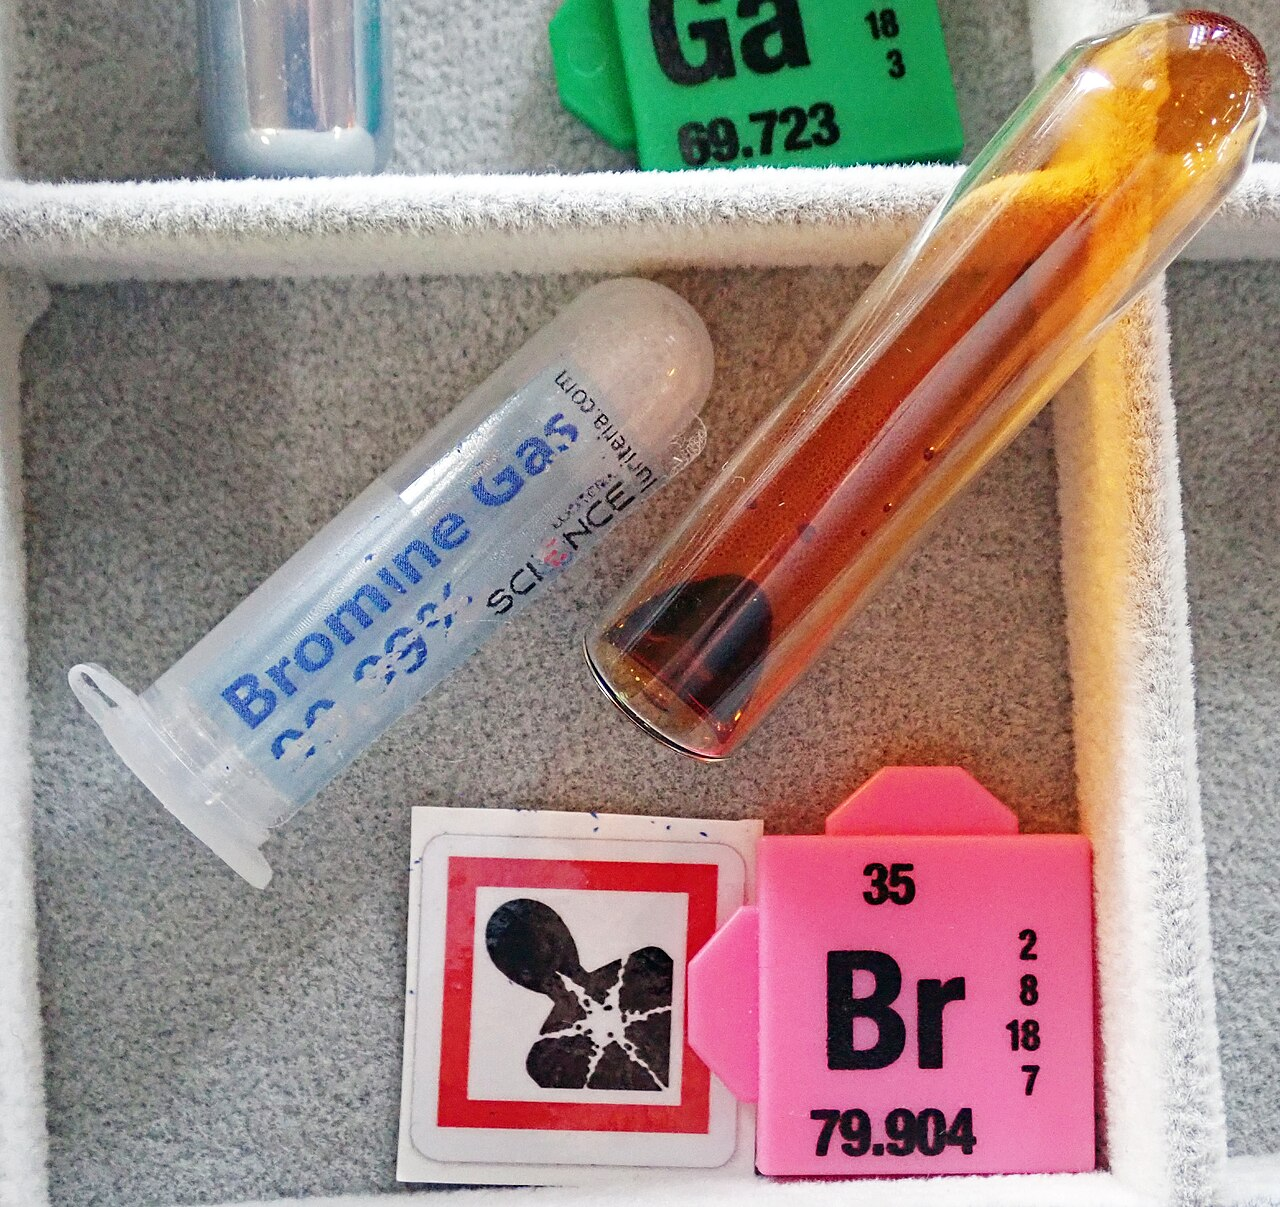
\includegraphics[width=0.4\linewidth, trim={585bp 418bp 15bp 130bp}, clip]
  {images/book1/bromine-gas.jpg}

{\small 大多数气体都看不见——但并非全部。这支密封的玻璃
管中装有溴，一种真正呈棕橙色的气体：你可以
\emph{看到}它充满容器的每一个角落，一直到
玻璃壁。\emph{Photo: James St.~John, CC BY 2.0 (cropped).}}
\end{omfigure}

\begin{remark}[分辨难辨的情形]\label{rem:g3:solids-liquids-gases:tricky}
有些东西需要仔细辨别。蜂蜜会流动——流得慢，但它仍在流动，
随容器改变形状，并保持体积：它是液体，
只不过是慢性子的液体。牙膏和番茄酱挤压时会流出：它们是稠厚的
液体。海绵是布满充气小孔的固体。烟呢？
细小的固体颗粒漂浮在热气体上。拿不准时，就问几个“家族”问题：
它能否保持形状？它能否流动？它能否充满
所给的全部空间？
\end{remark}

\section{练习}

\begin{exercise}[$\star$]\label{exo:g3:solids-liquids-gases:1}
将下列物质归入三个“家族”：一枚硬币；\ 橙汁；\ 轮胎内的
空气；\ 一颗木珠；\ 油；\ 沸腾的锅上方透明空隙处的
水蒸气。
\end{exercise}

\begin{exercise}[$\star$]\label{exo:g3:solids-liquids-gases:2}
固体能保持、而液体不能保持的是什么？液体
从玻璃杯倒入碗里时，又保持着什么？
\end{exercise}

\begin{exercise}[$\star$]\label{exo:g3:solids-liquids-gases:3}
将一整瓶柠檬水倒入宽口沙拉碗中。现在
柠檬水是变多了、变少了，还是一样多？变化的是什么？
\end{exercise}

\begin{exercise}[$\star$]\label{exo:g3:solids-liquids-gases:4}
画出一个装有半缸水的鱼缸：先平放，然后
一边抬起倾斜。两种情况下都画出水面——它
朝哪个方向？
\end{exercise}

\begin{exercise}[$\star$]\label{exo:g3:solids-liquids-gases:5}
建筑工人用的水平尺如何判断搁板是否水平？它
运用了本章的哪条定律？
\end{exercise}

\begin{exercise}[$\star$]\label{exo:g3:solids-liquids-gases:6}
为什么煎饼的香味能飘到楼上的卧室？是
哪一个“家族”在起作用？它的规则是什么？
\end{exercise}

\begin{exercise}[$\star$]\label{exo:g3:solids-liquids-gases:7}
沙子倾倒时像液体一样流动，但我们称它为固体。请
结合\cref{ex:g3:solids-liquids-gases:sand}加以解释。
\end{exercise}

\begin{exercise}[$\star$]\label{exo:g3:solids-liquids-gases:8}
蜂蜜需要整整一分钟才能从勺子上流下。它是固体
还是液体？请
依据\cref{rem:g3:solids-liquids-gases:tricky}中的“家族”问题作答。
\end{exercise}

\begin{exercise}[$\star$]\label{exo:g3:solids-liquids-gases:9}
哪一个“家族”：能保持自身形状？\ 随容器改变形状，但
保持体积不变？\ 会充满所能得到的全部空间？请分别举出
厨房中所见的每个“家族”各一例。
\end{exercise}

\begin{exercise}[$\star\star$]\label{exo:g3:solids-liquids-gases:10}
一块冰（固体）熔化成水（液体），夏日的阳光
又把水晒成看不见的飘动水汽（气体）。每一步
各打破了哪条“家族”规则？冰熔化时，物质不再保持什么？
水蒸发时呢？
\end{exercise}

\begin{exercise}[$\star\star$]\label{exo:g3:solids-liquids-gases:11}
气球吹大后扎紧了口。米拉说里面的空气是“
气球形的，所以气体确实有形状”。请解释真正
赋予形状的是什么，以及空气会
在气球爆破的那一瞬间怎样？
\end{exercise}
